\newpage
\section{EXISTING SYSTEM}
Tetris is a puzzle video game created by soviet software engineer Alexey Pajitnoovin 1984. It has been published by several companies for multiple platforms. The vanilla version of the game consisted of a board of dimension 10*18. It consisted of seven blocks of different shapes called tetromino blocks which were dropped continuously from the top of the board in a random order. It is this version of the game that we are taking as reference. The player has to smartly place each block in the board so as to fill a line. Filling a line will clear that particular row and all the blocks above that row will drop on that row. Blocks above this row will drop on this row and so on. Basically, the player has to prevent the board from filling otherwise the game will end displaying the final score. The vertical motion of the dropping block is automated and updates on each game tick so players cannot control the motion of the block along the column but they can rotate blocks in all directions and move them left and right along a row as they fall from the top. Blocks can’t be moved once they stop dropping. Players can also see the preview of the next block in the side window.
Today, Tetris can be found in a wide range of devices from PCs to mobile phones, with each adding new features to the already existing system.
\vfill
\begin{figure}[htb]
	\centering
	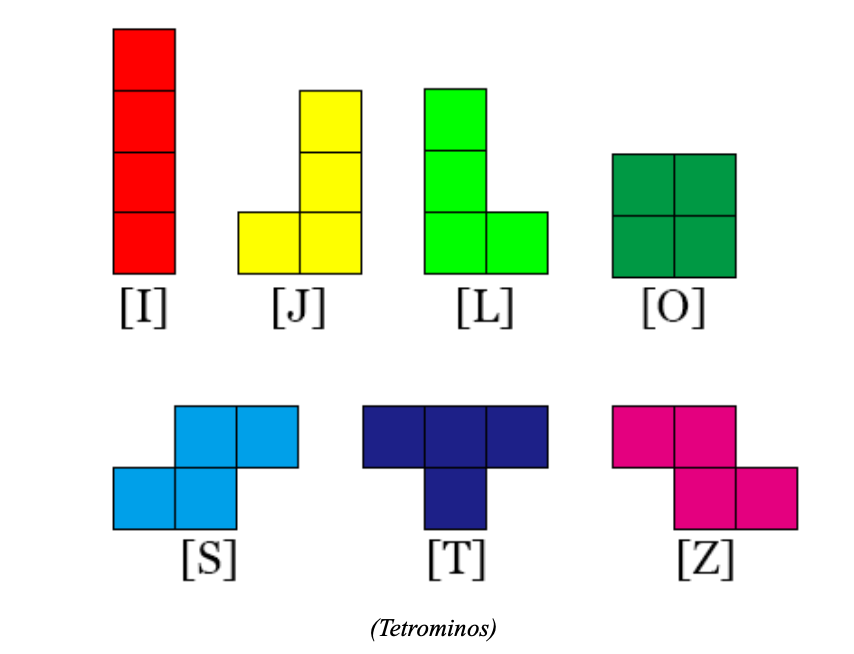
\includegraphics[width=0.9\textwidth]{images/Tetrominos.png}
\end{figure}
\vfill